\begin{figure}
  \centering
  \begin{subfigure}[t]{0.42\textwidth}
    \centering
    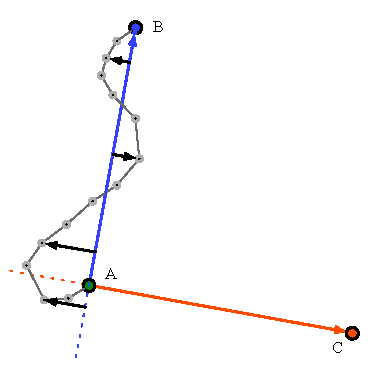
\includegraphics[width=\linewidth]{img/barycentric-spline.pdf}
    \caption{Spline primary points defined by stroke start ($A$) and
      end ($B$).}
    \label{fig:barycentric-spline}
  \end{subfigure}
  \hspace{1cm} % spacing, do what you need
  \begin{subfigure}[t]{0.42\textwidth}
    \centering
    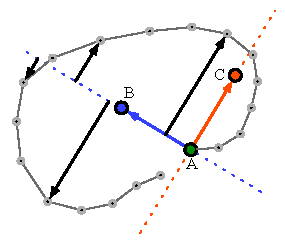
\includegraphics[width=\linewidth]{img/barycentric-blob.pdf}
    \caption{Blob primary points defined by stroke start ($A$) and
      initial centroid ($B$).}
    \label{fig:barycentric-blob}
  \end{subfigure}
  \caption[Spline and Blob Control Points]{Spline and Blob control
    points are defined in terms of two primary points, $A$ and $B$. A
    third point $C$ is simply B rotated 90 degrees about A. These
    points form the basis of a barycentric coordinate system. Control
    points are computed as a vector offset from $A$ in this coordinate
    space.}
  \label{fig:spline-blob-control-points}
\end{figure}

